\section{Elaboration}
%--------------------------------------------------------------------------------





\subsection{Abstractions}
%--------------------------------------------------------------------------------

$$
\Gamma \vdash \lambda x^A. e^E : R
$$

The type annotations $A$ and $E$ are optional.

An elaboration can be successful only if it elaborates a term which satifies the
requirement $R$. There are only two possibilities to satisfy the requirement.

\begin{enumerate}
    \item $R$ represents a function type i.e. it has the form $\Pi x^{A_r}.
        B_r$. In that case the requirement can flow down to give requirements
        for $A$, $E$ and $e$.

    \item $R$ has a metavariable $\meta M$ as a head term and $R$ is a pattern
        i.e. $R = \meta M \vec y$ where $\vec y$ are pairwise distinct free
        variables. In that case the requirement can flow up. I.e. the
        elaboration elaborates a term with the type $\Pi x^A. B$ and the
        unification of the type with $R$ instantiates $\meta M$.
\end{enumerate}


\begin{enumerate}
    \item $R = \Pi x^{A_r}. B_r$: I.e. the required type is a function type.

        \begin{enumerate}
            \item If $A$ is present then elaborate $A$ with $\Gamma \vdash A_r
                \le A$. Otherwise use $A = A_r$.

            \item If $E$ is present then elaborate $E$
                with $\Gamma, x^A \vdash E \le B_r$. Otherwise use $E = B_r$.

            \item Elaborate $e$ with $\Gamma, x^A \vdash e: E$.

            \item Form $\Gamma \vdash \lambda x^A. e^E : \Pi x^A. E$ where $\Pi
                x^A. E$ is guaranteed to be a subtype of $\Pi x^{A_r}. B_r$.

                The forming of $\lambda x^A. e^E$ requires that all
                metavariables belonging to the context $\Gamma, x^A$ are
                instantiated. This usually requires waiting (e.g. $e$ is usually
                an application where the metavariables representing arguments
                have to be instantiated).
        \end{enumerate}

    \item $R = \meta M \vec a$: The required type is represented by an
        uninstantiated metavariable $\meta M$.

    \item All other cases are error cases.

        Open question: What happens with a stuck case tree application?
\end{enumerate}





\subsection{Applications}
%---------------------------------------------------------------------------

$$ f a$$


The elaborator of $f a$ starts with a signature requirement $[R]$ and
an optional required type.

\paragraph{Subtasks}
\begin{enumerate}
    \item $E_f$: Elaborate $f$
    \item $E_a$: Elaborate $a$
    \item $U_{A}$: Unify the type of $a$ as a subtype of the argument type of
        $f$
    \item $U_{R}$: Unify the type of $\meta f \meta a$ as a subtype of the
        required type of $fa$.
    \item $E_{fa}$: Elaborate $fa$
\end{enumerate}

The subtasks $E_f$, $U_A$, $U_R$ and $E_{fa}$ have to be executed in sequence. The
subtask $E_a$ can run interleaved.


\paragraph{Algorithm}
\begin{enumerate}
    \item Make holes:
        \begin{enumerate}
            \item Make the unkown signature element $\meta U$.

            \item Make a hole $\meta f$ for $f$ with signature requirement $[\meta U, R]$.

            \item Make a hole $\meta A$ for the type of $a$ with the signature
                requirement $[S]$.

            \item Make a hole $\meta a$ for $a$ with signature requirement $[\meta U]$
                and the
                required type $\meta A$.
        \end{enumerate}

    \item Waiting tasks:
        \begin{enumerate}
            \item Put $U_{A}$ into the wait queue for $\meta f$.

            \item Put $U_R$ into the wait queue for $U_A$.

            \item Put $E_{fa}$ into the wait queue for $U_R$.
        \end{enumerate}

    \item Ready tasks:
        \begin{enumerate}
            \item Push $E_a$ into the ready queue.

            \item Push $E_f$ into the ready queue.
        \end{enumerate}
\end{enumerate}


\paragraph{Remarks}

\begin{itemize}
    \item The elaborators of $f$ and $a$ don't have any preconditions. For the
        result of the elaboration the sequence is not important. However it is
        preferable to start the elaboration of $f$ before the elaboration of
        $a$. The elaboration of $a$ has a better chance to be successful without
        becoming stuck if the elaboration of $f$ has finished and the required
        type $\meta A$ for $a$ is available.

    \item The term $fa$ can be built as soon as the type of $a$ is unified with
        the argument type of $f$ and the type of $\meta f \meta a$ is unified
        with the required result type. Before that it is not evident that $fa$ is
        welltyped and satisfies its requirement.
\end{itemize}




\paragraph{Example}
%------------------------------------------------------------
Elaborate the term
\begin{alba}
    (|>) 1 (+) 2: Nat

    -- equivalent to
    (1 |> (+)) 2: Nat

    -- in global context
    (+): Nat -> Nat -> Nat
    (+): String -> String -> String)

    (|>) {A: Any} {P: A -> Any} (a: A) (f: all x: P x): P a
    :=
        f a
\end{alba}

\resizebox{8cm}{3cm}{
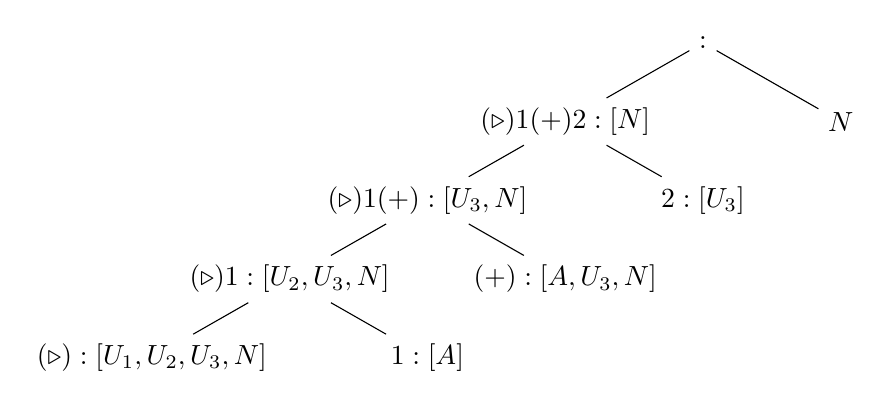
\begin{tikzpicture}
    \def\app{{\scriptsize app}}
    \def\f{{(\triangleright)}}
    \def\p{{(+)}}
    \node {:} [sibling distance = 3.5cm, level distance = 1cm]
        child {node {$\f 1 \p 2:[N]$}
            child {node {$\f 1 \p:[U_3, N]$}
                child {node {$\f 1:[U_2, U_3, N]$}
                    child {node {$\f: [U_1,U_2,U_3,N]$}}
                    child {node {$1: [A]$}}
                }
                child {node {$(+): [A,U_3,N]$}}
            }
            child {node {$2: [U_3]$}}
        }
        child {node {$N$}};
\end{tikzpicture}
}

We start with the elaboration of $(\triangleright) 1 (+) 2$ with the signature
requirement $[N]$ and the required type $N$.

\begin{itemize}
    \item The term is an application with the function term $(\triangleright) 1
        (+)$ and the argument $2$. We start the elaboration of the function term
        with the signature requirement $[U_3, N]$ and no required type.

    \item The term is again an application with the function term
        $(\triangleright) 1$ and the argument $(+)$. We start the elaboration
        of the function term with the signature requirement $[U_2, U_3, N]$ and
        no required type.

    \item The term is again an application with the function term
        $(\triangleright)$ and the argument $1$. We start the elaboration of the
        function term with the signature requirement $[U_1, U_2, U_3, N]$ and no
        required type.

    \item The term $(\triangleright)$ is a global name with the signature $[I,
        I, A, [A, P], P]$. Unification with the required signature $[U_1, U_2,
        U_3, N]$ results in
        $$
        \begin{array}{lll}
            U_1 &:=& A
            \\
            U_2 &:=& [A, U_3, N]
            \\
            P   &:=& [U_3, N]
        \end{array}
        $$
        Because of the two implicit arguments the term is elaborated as
        $(\triangleright)A P$ with the metavariables $A$ and $P$.

    \item Next the argument term $1$ has to be elaborated with the required
        signature $[A]$ and the required type $A$. This elaboration gets stuck
        on $A$, because the elaborator cannot decide the number type.

    \item Next the argument term $(+)$ is tried with the required signature $[A,
        U_3, N]$. The global name is ambiguous, but the ambiguity can be
        resolved by the result type. The signature is $[N, N, N]$. Unification
        with the required signature results in
        $$
        \begin{array}{lll}
            A &:=& N
            \\
            U_3 &:=& N
        \end{array}
        $$

    \item Now the complete term can be elaborated as
        $$
            (\triangleright) N (N \to N) \meta a (+) \meta b
        $$
        leaving the two holes $\meta a$ and $\meta b$ for the remaining
        arguments. However by unification the metavariables $\meta A$ and $\meta
        U_3$ are instantiated by $N$ and therefore the elaboration of the
        remaining arguments is unblocked and finally will succeed.
\end{itemize}
